%Copyright 2014 Jean-Philippe Eisenbarth
%This program is free software: you can 
%redistribute it and/or modify it under the terms of the GNU General Public 
%License as published by the Free Software Foundation, either version 3 of the 
%License, or (at your option) any later version.
%This program is distributed in the hope that it will be useful,but WITHOUT ANY 
%WARRANTY; without even the implied warranty of MERCHANTABILITY or FITNESS FOR A 
%PARTICULAR PURPOSE. See the GNU General Public License for more details.
%You should have received a copy of the GNU General Public License along with 
%this program.  If not, see <http://www.gnu.org/licenses/>.

%Based on the code of Yiannis Lazarides
%http://tex.stackexchange.com/questions/42602/software-requirements-specification-with-latex
%http://tex.stackexchange.com/users/963/yiannis-lazarides
%Also based on the template of Karl E. Wiegers
%http://www.se.rit.edu/~emad/teaching/slides/srs_template_sep14.pdf
%http://karlwiegers.com
\documentclass[oneside,a4paper,12pt,explicit]{book}
% adapted and reformated from https://www.overleaf.com/latex/templates/msa-cs-software-requirement-specification-document/gdbzgspvjqqz
\usepackage[utf8]{inputenc}
\usepackage[sedes]{kultem}
\usepackage[english]{babel}
\usepackage{mdframed}
\usepackage{csquotes} % for compilation error
\usepackage[backend=bibtex, style=ieee]{biblatex} % You can change 'numeric' to 'ieee' or 'apa' if you want
\addbibresource{references.bib} % This points to your .bib file


%% INSERT YOUR PACKAGES HERE
\usepackage[accsupp]{axessibility}% improves PDF readability for those with disabilities.
\usepackage[hidelinks]{hyperref}
\usepackage{lipsum}
\usepackage{imakeidx}
\makeindex
\usepackage{float}
\usepackage{listings}
\usepackage{tabularx}
\usepackage{adjustbox}
\usepackage{subcaption}
\setlength{\headheight}{15pt} % to avoid compiler warnings
\renewcommand{\arraystretch}{1.2} % Adjust row height for better readability
%% TITLE PAGE OPTIONS (only works with \maketitle is called in the document)
\title{Project of AAA Furnitures}
\subtitle{Software Requirement Specification}
\date{\today}
\author{Andreandhiki Riyanta Putra\\Andrian Danar Perdana\\M. Argya Vityasy}
\professor{Khabib Mustofa}
\status{DRAFT adapted from \href{https://dspmuranchi.ac.in/pdf/Blog/srs_template-ieee.pdf}{IEEE SRS Template}}
\version{1.0}

%% DOCUMENT
\begin{document}
\maketitle
\large
\tableofcontents
\normalsize
\chapter*{Revision History}

\begin{center}
    \begin{tabular}{|c|c|c|c|}
        \hline
	    Name & Date & Reason For Changes & Version\\
        \hline
	    21 & 22 & 23 & 24\\
        \hline
	    31 & 32 & 33 & 34\\
        \hline
    \end{tabular}
\end{center}

\chapter{Introduction}

\section{Purpose}
The purpose of this document is to present a detailed description of the functional
and non-functional requirements for the Furniture Selling Web Based Application.
It will also explain the app constraints, interface, and interactions with each services.
This document is intended for both the stakeholders and the developers
for a reference of developing the first version of the application.

\section{Project Scope}
AAA Furnitures is a web-based application that allows the customers of AAA Furnitures 
to purchase furnitures online. The application will allow the customers 
to browse the available furnitures, add them to the cart,
make secure payments, and track the delivery of the purchased items.
The application will also allow the admin to manage the products displayed on the website 
and the orders made by the customers.
The system will consist of multiple microservices, including the auth service, product service,
the order service, the payment service, and the delivery service.


\section{Definitions, Acronyms, and Abbreviations}
\begin{table}[H]
    \centering
    \renewcommand{\arraystretch}{1.2} % Adjust row height for better readability
    \begin{tabularx}{\textwidth}{|l|X|}
        \hline
        \textbf{Term} & \textbf{Definition} \\
        \hline
        User & A registered customer who can browse, add to cart, and place orders. \\
        \hline
        Admin & A user with special privileges to manage products, orders, and the contact for users. \\
        \hline
        Cart & A temporary collection of items selected by a user for purchase. \\
        \hline
        Order & A confirmed request for purchasing one or more items. \\
        \hline
        JWT & JSON Web Token, used for authentication and authorization. Used for the user login, logout\cite{rfc7519}  \\
        \hline
        API & Application Programming Interface, allows different services to communicate with each other.\cite{API}\\
        \hline
        REST & Representational State Transfer, an architectural style for designing APIs that use stateless communication over HTTP.\cite{REST} \\
        \hline
        Session & A temporary authentication state that maintains user login status. \\
        \hline
        SQL & Structured Query Language, used for managing relational databases by defining, querying, and modifying data.\cite{SQL}\\
        \hline
        Microservice & An architectural style that structures an application as a collection of small, independent, and loosely coupled services.\cite{9282637} \\
        \hline
        Message Queueing & A communication method where messages are sent and stored in a queue, ensuring asynchronous processing between microservices such as order, delivery, and payment services.\cite{Bouchenak2009}\\
        \hline
    \end{tabularx}
    \caption{Definitions, Acronyms, and Abbreviations}
    \label{tab:definitions}

\end{table}

\section{References}
\printbibliography[heading=none]

\chapter{Overall Description}

\section{Product Perspective}
This product is a new e-commerce platform designed as a microservices-based system. 
It aims to provide a comprehensive online shopping experience with user authentication,
product browsing, order management, payment processing, and delivery tracking capabilities.
The system is self-contained but designed with a modular architecture to allow for future expansion
and integration with third-party services such as payment gateways and shipping providers. 
The microservices architecture ensures that each component can be developed, deployed, and scaled independently.

The following figure \ref{fig:architecture} illustrates the high-level architecture of the system:

\begin{figure}[H]
    \centering
    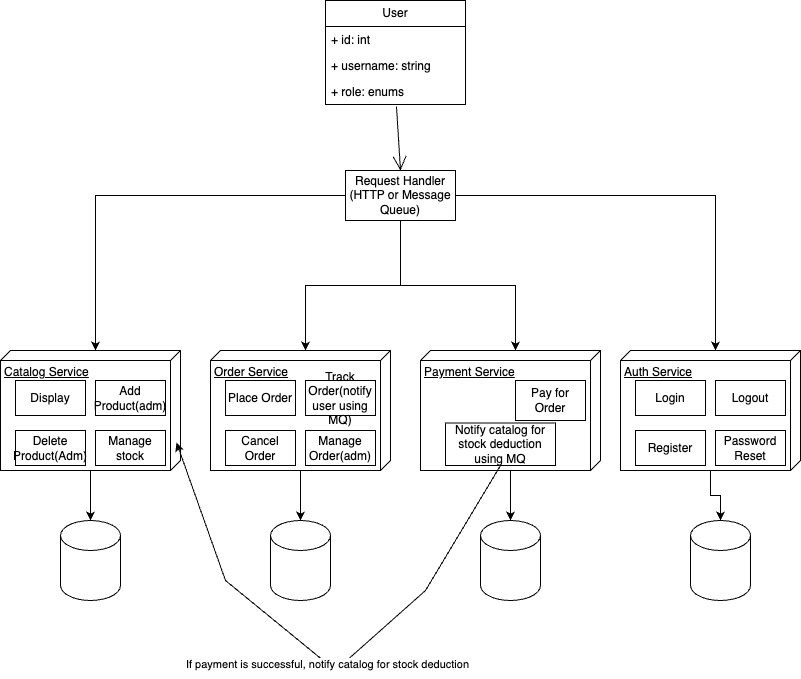
\includegraphics[width=0.8\textwidth]{img/app diagram.drawio.png}
    \caption{System Architecture Diagram}
    \label{fig:architecture}
\end{figure}
\section{Product Functions}
The e-commerce platform will perform the following major functions:

\begin{itemize}
    \item User Authentication and Account Management
    \begin{itemize}
        \item Register new user accounts
        \item Login and logout functionality
        \item Password reset capabilities
    \end{itemize}
    
    \item Product Catalog Management
    \begin{itemize}
        \item Browse and display product information
        \item Add new products (administrator function)
        \item Delete products (administrator function)
        \item Manage product inventory
    \end{itemize}
    
    \item Order Processing
    \begin{itemize}
        \item Add products to shopping cart
        \item Place and confirm orders
        \item Cancel existing orders
        \item Track order status and delivery
    \end{itemize}
    
    \item Payment Processing
    \begin{itemize}
        \item Process secure payments for orders
        \item Notify catalog service for inventory updates
    \end{itemize}
    
    \item Delivery Management
    \begin{itemize}
        \item Arrange delivery for completed orders
        \item Track delivery status
    \end{itemize}
\end{itemize}
Figure \ref{fig:usecase} illustrates the use case for this application:
\begin{figure}[H]
    \centering
    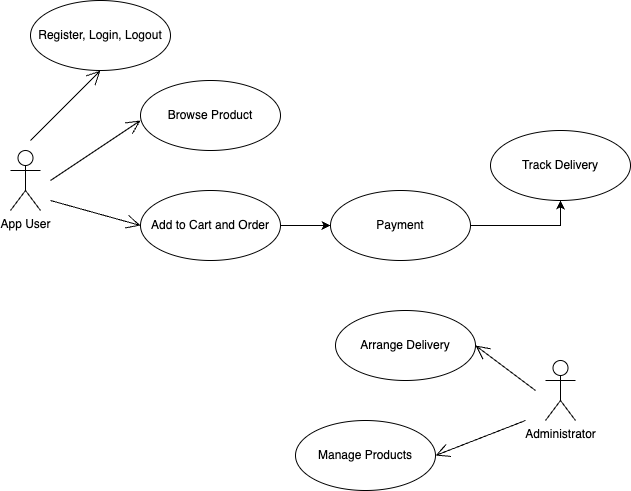
\includegraphics[width=0.5\textwidth]{img/users diagram.drawio (1).png}
    \caption{Use Case Diagram}
    \label{fig:usecase}
\end{figure}

\section{User Classes and Characteristics}
The system will serve the following user classes:

\begin{itemize}
    \item Regular App Users
    \begin{itemize}
        \item Frequency: Regular, potentially daily use
        \item Functions: Browse products, manage cart, place orders, track deliveries
        \item Technical expertise: Minimal, should be able to navigate standard e-commerce interfaces
        \item Priority: High - primary user class
    \end{itemize}
    
    \item Administrators
    \begin{itemize}
        \item Frequency: Regular, primarily during business hours
        \item Functions: Manage product catalog, arrange deliveries, handle order issues
        \item Technical expertise: Moderate, trained on system administration
        \item Security level: High, with access to user data and system configuration
        \item Priority: Medium - essential for system operation but smaller user base
    \end{itemize}
    
    \item Guest Users
    \begin{itemize}
        \item Frequency: Occasional to one-time use
        \item Functions: Browse products only, limited functionality until registration
        \item Technical expertise: Minimal
        \item Priority: Low - encourage conversion to registered users
    \end{itemize}
\end{itemize}

\section{Operating Environment}
The software will operate in the following environment:

\begin{itemize}
    \item Server Environment
    \begin{itemize}
        \item Containerized microservices using Docker
        \item Kubernetes for orchestration
        \item Linux-based operating systems
        \item Scalable cloud infrastructure (AWS, Google Cloud, or Azure)
    \end{itemize}
    
    \item Client Environment
    \begin{itemize}
        \item Web browser support: Chrome, Firefox, Safari, Edge (latest versions)
        \item Responsive design for various screen sizes
    \end{itemize}
    
    \item Database Environment
    \begin{itemize}
        \item Dedicated database for each microservice as shown in the architecture diagram
        \item Support for SQL and NoSQL databases depending on service requirements
    \end{itemize}
    
    \item Network Environment
    \begin{itemize}
        \item HTTP/HTTPS protocols for client-server communication
        \item Message Queue (MQ) for asynchronous inter-service communication
    \end{itemize}
\end{itemize}

\section{Design and Implementation Constraints}
The following constraints will affect the design and implementation of the system:

\begin{itemize}
    \item Architectural Constraints
    \begin{itemize}
        \item Microservices architecture as depicted in the diagram
        \item RESTful API design principles for service interfaces
        \item Message Queue for asynchronous communication between services
    \end{itemize}
    
    \item Security Constraints
    \begin{itemize}
        \item Compliance with PCI DSS for payment processing
        \item Secure user authentication and authorization
        \item Data encryption for sensitive information
        \item Safe payment for user
        \item Regular security audits and penetration testing
    \end{itemize}
    
    \item Integration Constraints
    \begin{itemize}
        \item Compatible with standard payment gateways
        \item API-based integration with shipping and delivery services
    \end{itemize}
    
    \item Performance Constraints
    \begin{itemize}
        \item Response time for user interactions under 2 seconds
        \item System capable of handling at least 1000 concurrent users
        \item Scalability to accommodate peak shopping seasons
    \end{itemize}
    
    \item Development Constraints
    \begin{itemize}
        \item Coding standards and style guides for consistency
        \item Comprehensive unit and integration testing
        \item CI/CD pipeline for automated testing and deployment
    \end{itemize}
\end{itemize}

\section{Assumptions and Dependencies}
The following assumptions and dependencies apply to the project:

\begin{itemize}
    \item Assumptions
    \begin{itemize}
        \item Users have access to stable internet connections
        \item Peak usage will occur during promotional events and holidays
        \item Most users will access the system via mobile devices
        \item Inventory data will be updated in near real-time
    \end{itemize}
    
    \item Dependencies
    \begin{itemize}
        \item Reliable third-party payment processing services
        \item Shipping and delivery partner APIs
        \item Cloud infrastructure provider's uptime and service level agreements
        \item Message Queue service for inter-service communication
        \item Database management systems for each service's data storage
    \end{itemize}
    x
    \item Risks
    \begin{itemize}
        \item Integration challenges with third-party services
        \item Scalability issues during peak usage periods
        \item Security vulnerabilities in payment processing
        \item Data consistency across microservices
    \end{itemize}
\end{itemize}

\chapter{External Interface Requirements}

\section{User Interfaces}
$<$Describe the logical characteristics of each interface between the software 
product and the users. This may include sample screen images, any GUI standards 
or product family style guides that are to be followed, screen layout 
constraints, standard buttons and functions (e.g., help) that will appear on 
every screen, keyboard shortcuts, error message display standards, and so on.  
Define the software components for which a user interface is needed. Details of 
the user interface design should be documented in a separate user interface 
specification.$>$
\begin{figure}[H]
    \centering
    \begin{minipage}{0.4\textwidth}
        \centering
        \fbox{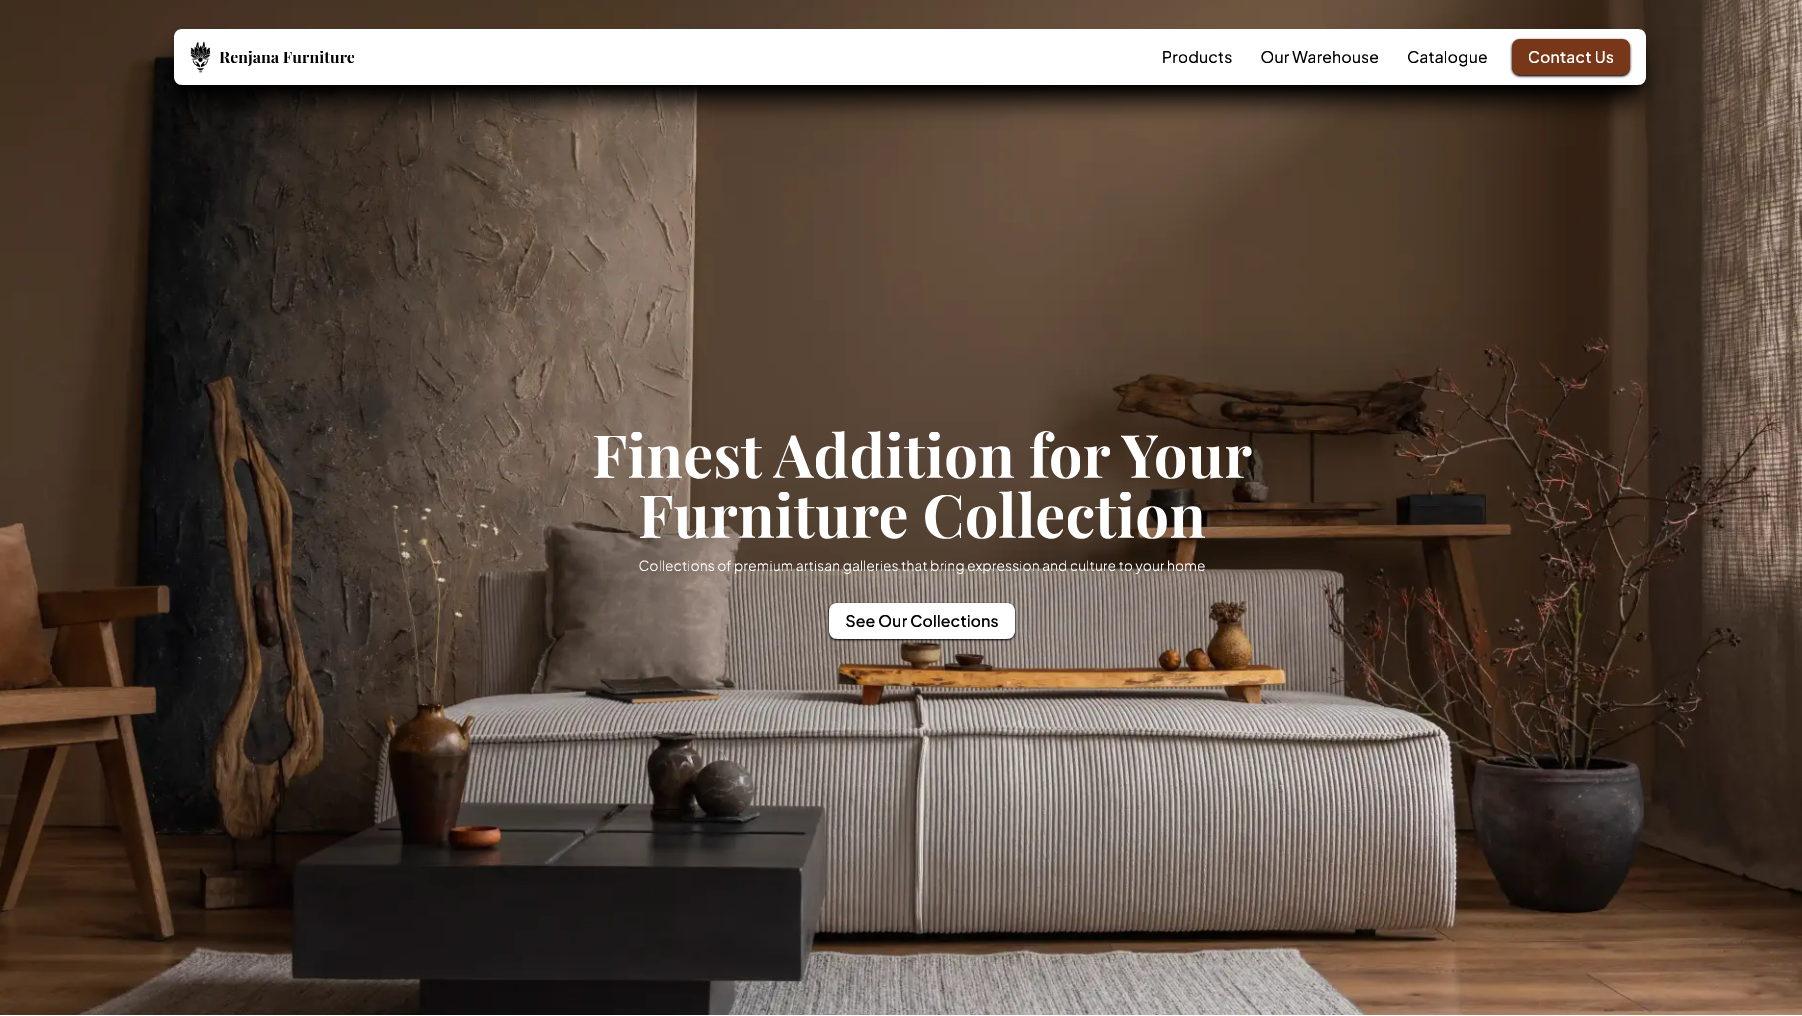
\includegraphics[width=\linewidth]{img/ui/landingpage-1.png}}
        \caption{Hero Section}
    \end{minipage}
    \hfill
    \begin{minipage}{0.5\textwidth}
        \centering
        \fbox{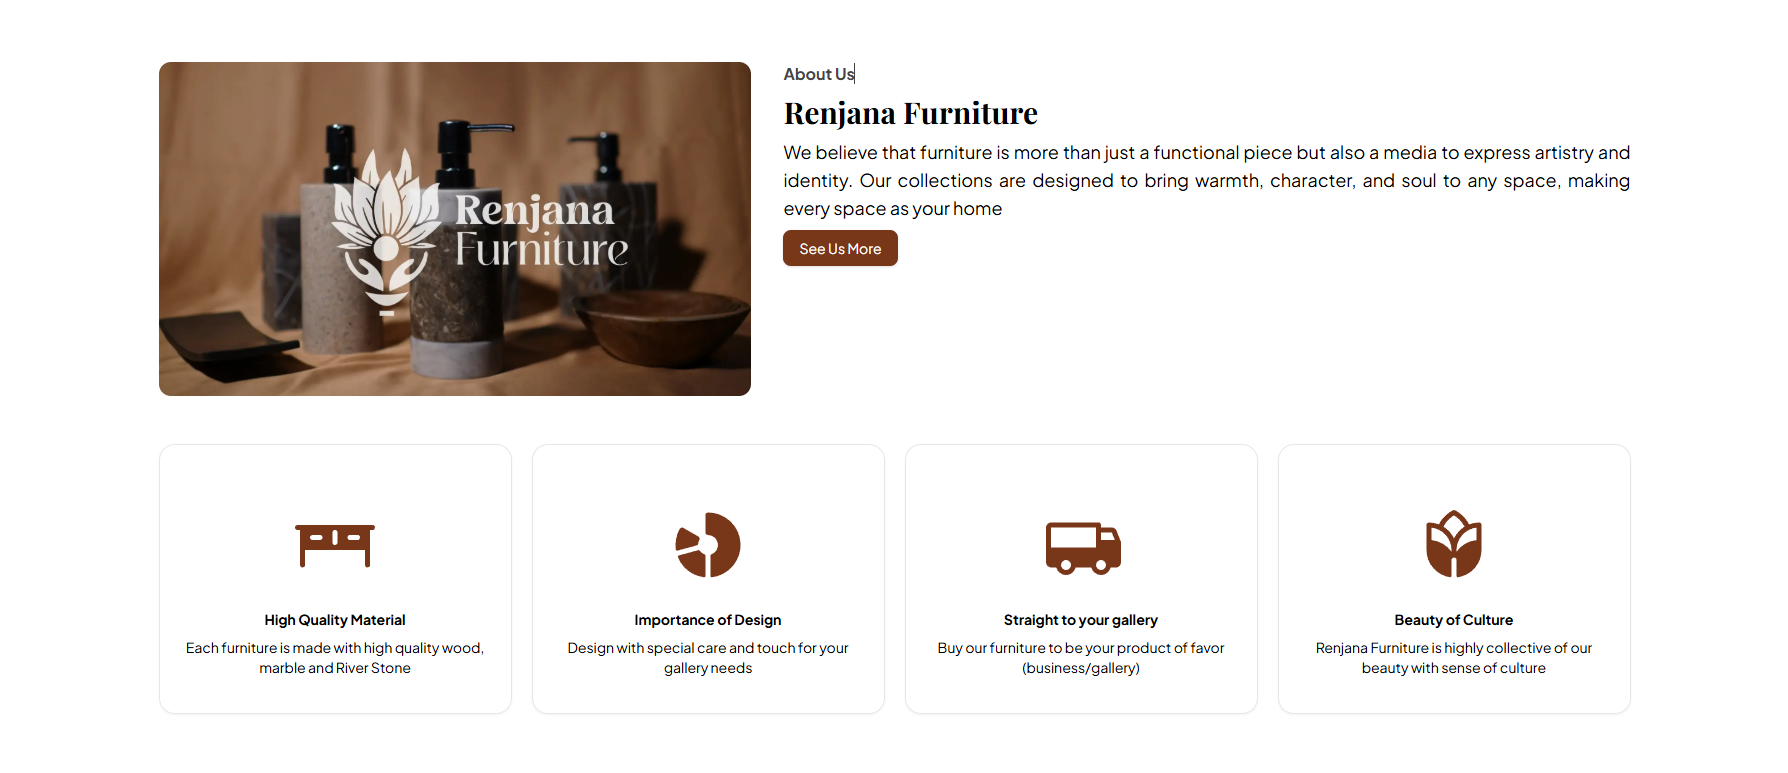
\includegraphics[width=\linewidth]{img/ui/landingpage-2.png}}
        \caption{About Section}
    \end{minipage}
\end{figure}
\begin{figure}[H]
    \centering
    \begin{minipage}{0.4\textwidth}
        \centering
        \fbox{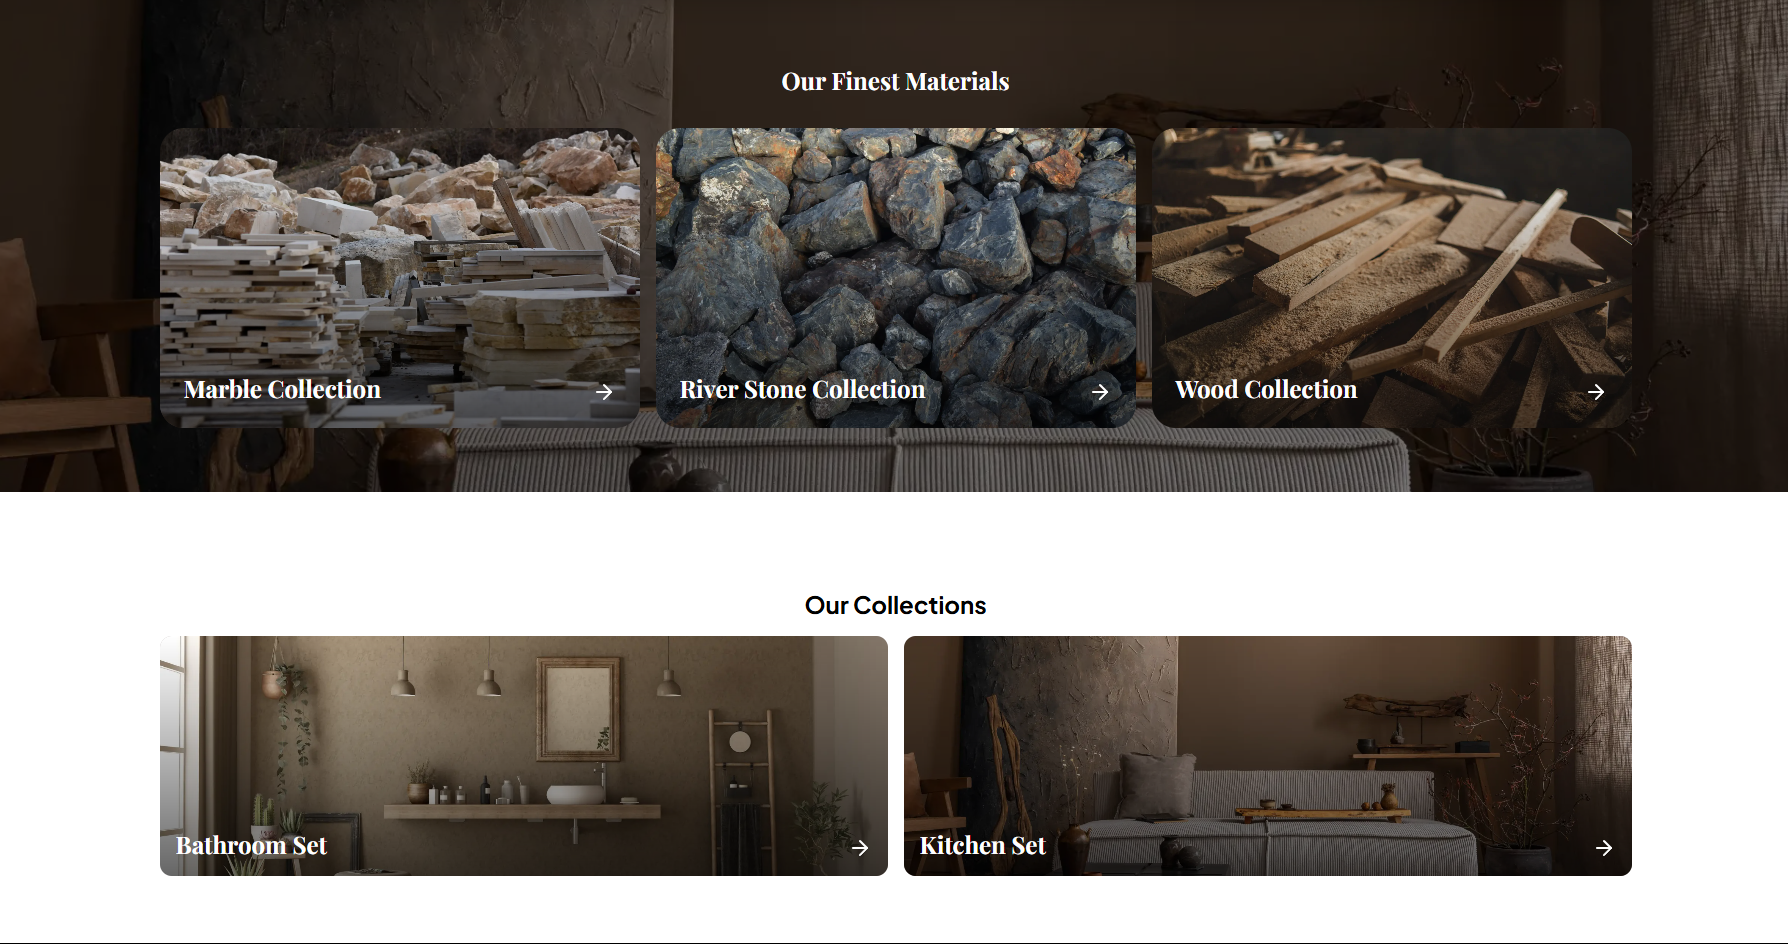
\includegraphics[width=\linewidth]{img/ui/landingpage-3.png}}
        \caption{Hero Section}
    \end{minipage}
    \hfill
    \begin{minipage}{0.5\textwidth}
        \centering
        \fbox{
\includegraphics[width=\linewidth]{img/ui/landingpage-4.png}}
        \caption{About Section}
    \end{minipage}
\end{figure}

\begin{figure}[H]
    \centering
    \begin{minipage}{0.48\textwidth}
        \centering
        \fbox{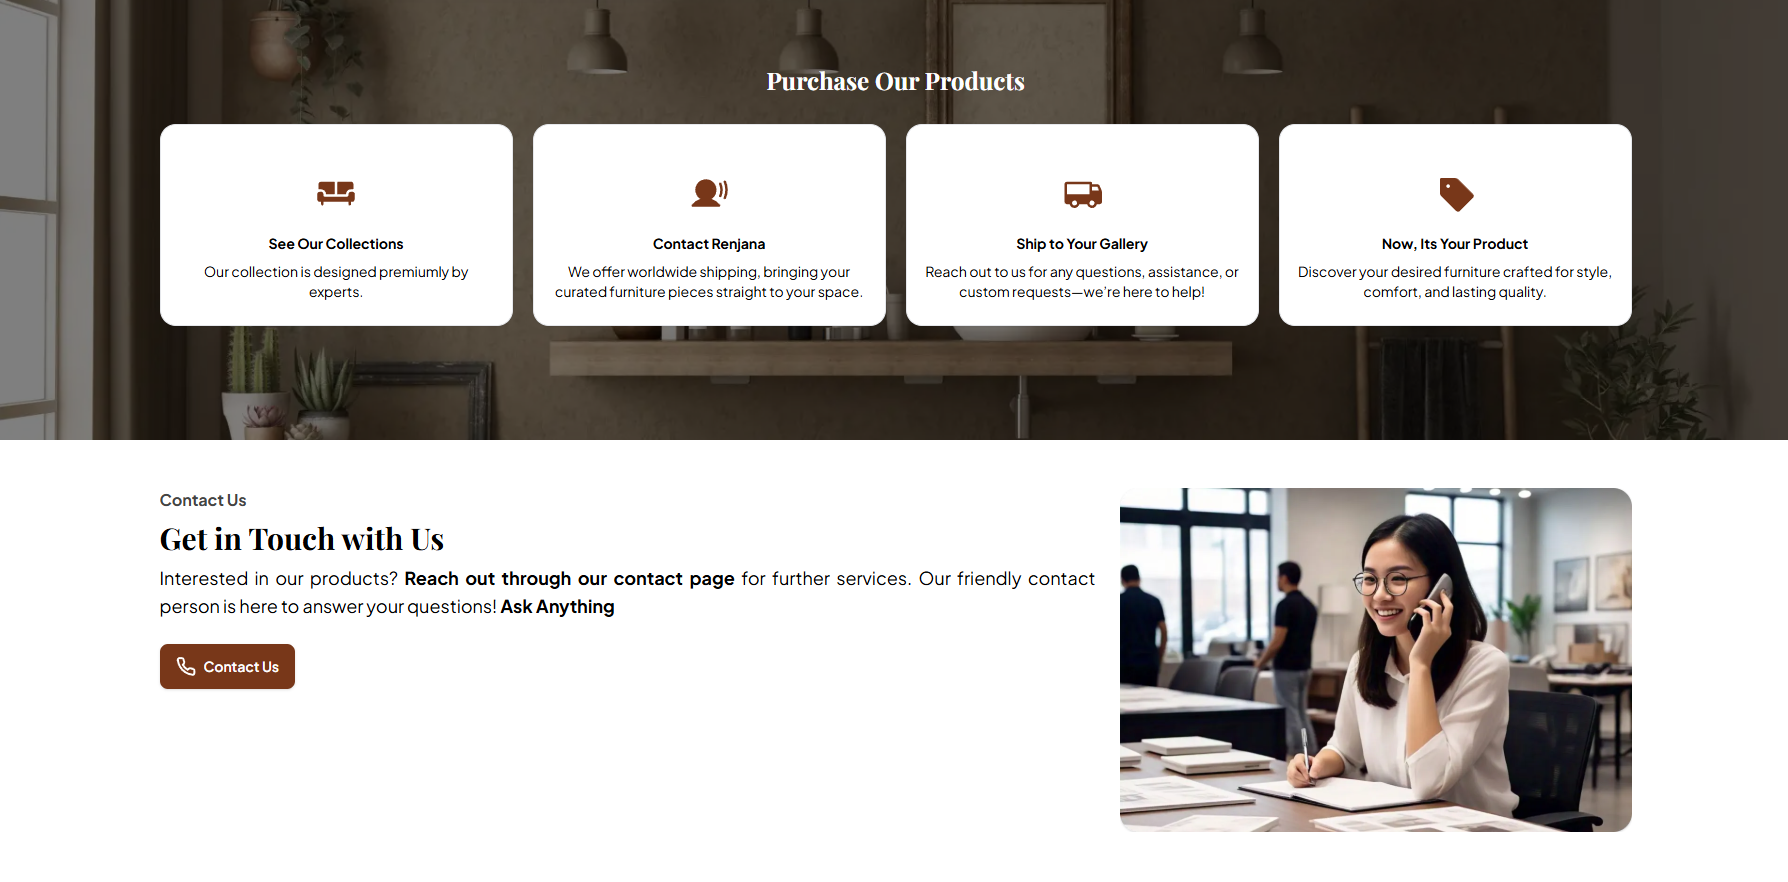
\includegraphics[width=\linewidth]{img/ui/landingpage-5.png}}
        \caption{Hero Section}
    \end{minipage}
    \hfill
    \begin{minipage}{0.44\textwidth}
        \centering
        \fbox{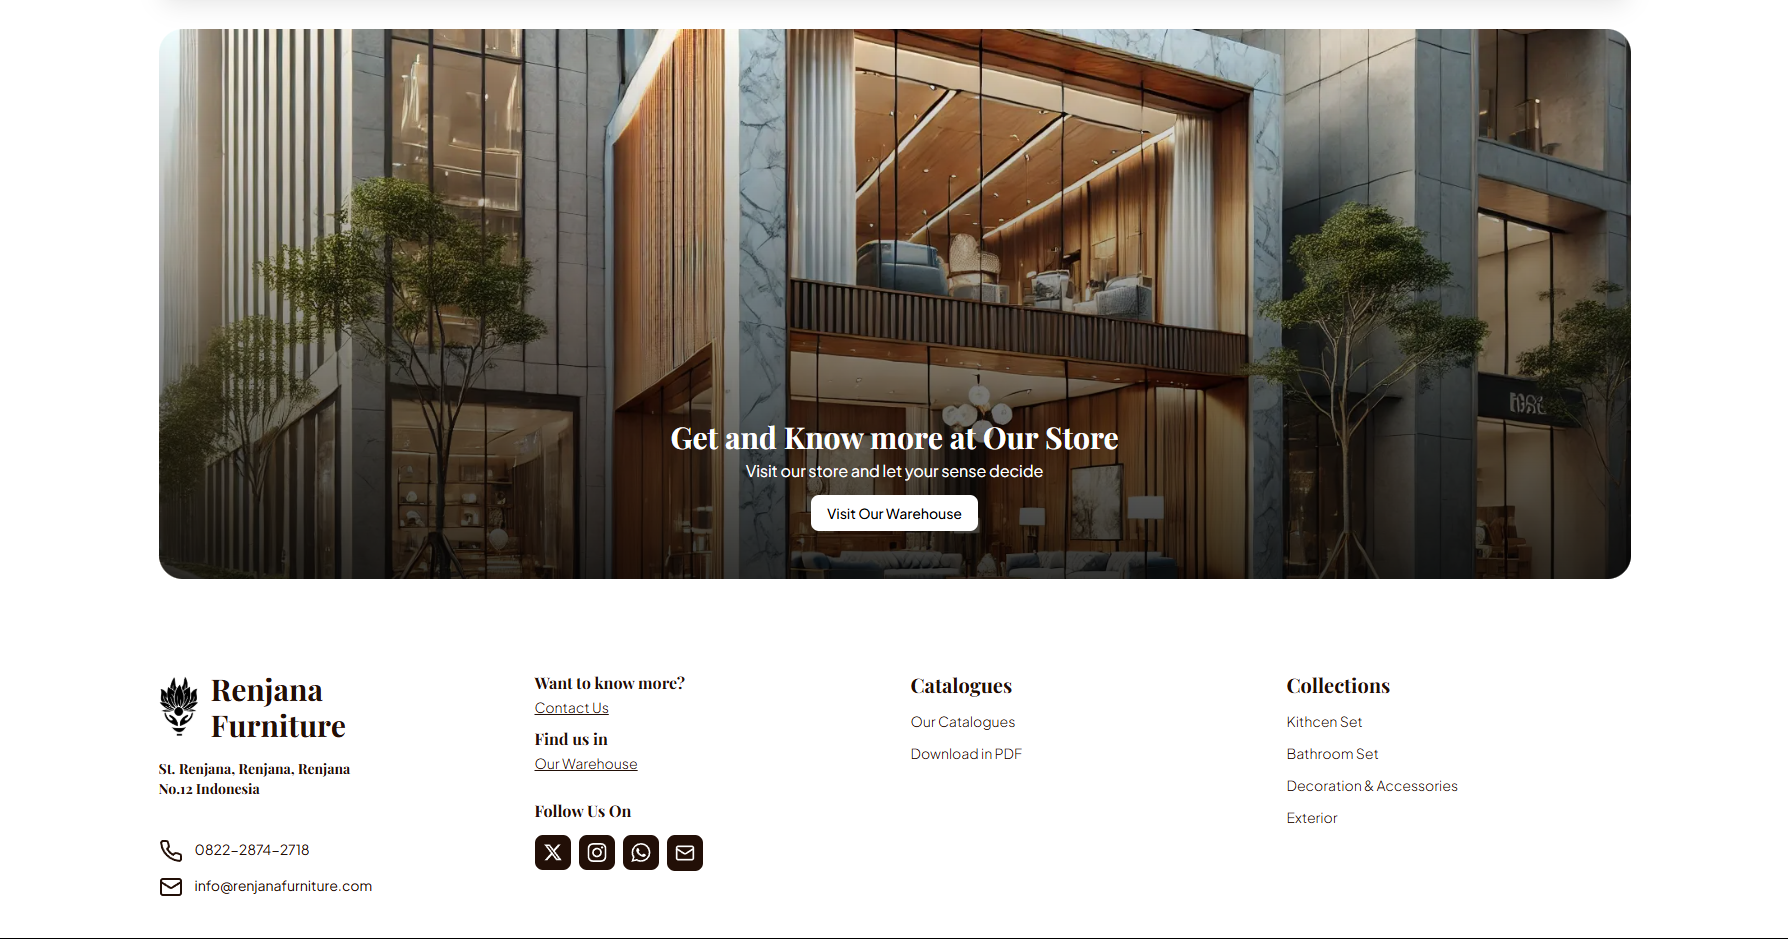
\includegraphics[width=\linewidth]{img/ui/landingpage-6.png}}
        \caption{About Section}
    \end{minipage}
\end{figure}


% Done
\section{Hardware Interfaces}
The catalog website and the admin dashboard do not depend on specific hardware components, and therefore, no direct hardware interfaces are required. All product-related data, including images, descriptions, and other relevant details, are managed within the web platform. Payment transactions are facilitated through direct communication via WhatsApp rather than a dedicated payment processing hardware.

The database server connection is handled by the underlying infrastructure provided by the hosting service, ensuring reliable data storage and retrieval for both visitors and administrators. This approach abstracts hardware dependencies, allowing the system to operate efficiently across various environments.

% Done
\section{Software Interfaces}
The catalog website interacts with various software components to ensure seamless functionality and efficient data management. It is developed using Next.js as the primary frontend framework, with Tailwind CSS for styling and responsive design. The backend is managed through Payload CMS, which facilitates content organization and retrieval.

The system utilizes Supabase (Vercel Postgres) as its primary database for storing product details, user interactions, and other relevant data. Additionally, Supabase storage is used to handle and serve product images, ensuring optimized retrieval and delivery. Communication between the frontend and backend occurs via API requests, allowing structured data exchange and synchronization.

For transactions, the website does not include an integrated payment gateway but instead facilitates purchases through direct WhatsApp messaging. Furthermore, third-party libraries and services are integrated for image optimization, SEO enhancements, and performance monitoring to improve user experience and website visibility.

Data sharing between software components follows an API-driven approach, ensuring security, consistency, and scalability. If required, additional implementation constraints, such as authentication mechanisms and rate limiting, can be applied to protect data integrity.

% Done
\section{Communications Interfaces}
The catalog website relies on standard web communication protocols to ensure seamless data exchange between the frontend, backend, and external services. The system primarily uses HTTPS for secure communication and is accessible through modern web browsers.

Data transactions between the frontend and backend are managed through GraphQL API provided by Payload CMS, allowing efficient retrieval and management of product information stored in Supabase (Vercel Postgres).

For customer inquiries via the Contact Us form, the system integrates with Google Sheets API to store submitted form data in a centralized Google Sheet. Additionally, Nodemailer is used to send email notifications based on form submissions, ensuring that administrators are promptly informed of customer inquiries.

To enhance the user experience, the website also integrates Google Maps API, which provides an interactive map displaying the warehouse location. This allows users to easily locate the company's physical store or storage facility.

Since transactions are conducted outside the platform via WhatsApp messaging, no payment gateway integration is required. WhatsApp's built-in encryption ensures secure communication between customers and the business.

To maintain data integrity and security, all API communications follow industry best practices, including authentication mechanisms, rate limiting, and encrypted data transmission where applicable.

\chapter{System Features}
% Upper Bound
% $<$This template illustrates organizing the functional requirements for the 
% product by system features, the major services provided by the product. You may 
% prefer to organize this section by use case, mode of operation, user class, 
% object class, functional hierarchy, or combinations of these, whatever makes the 
% most logical sense for your product.$>$

% \section{System Feature 1}
% $<$Don’t really say “System Feature 1.” State the feature name in just a few 
% words.$>$

% \subsection{Description and Priority}
% $<$Provide a short description of the feature and indicate whether it is of 
% High, Medium, or Low priority. You could also include specific priority 
% component ratings, such as benefit, penalty, cost, and risk (each rated on a 
% relative scale from a low of 1 to a high of 9).$>$

% \subsection{Stimulus/Response Sequences}
% $<$List the sequences of user actions and system responses that stimulate the 
% behavior defined for this feature. These will correspond to the dialog elements 
% associated with use cases.$>$

% \subsection{Functional Requirements}
% $<$Itemize the detailed functional requirements associated with this feature.  
% These are the software capabilities that must be present in order for the user 
% to carry out the services provided by the feature, or to execute the use case.  
% Include how the product should respond to anticipated error conditions or 
% invalid inputs. Requirements should be concise, complete, unambiguous, 
% verifiable, and necessary. Use “TBD” as a placeholder to indicate when necessary 
% information is not yet available.$>$

% $<$Each requirement should be uniquely identified with a sequence number or a 
% meaningful tag of some kind.$>$

% REQ-1:	REQ-2:

% Lower Bound

\section{Product Management}

\subsection{Description and Priority}
This feature enables administrators to efficiently manage the product catalog by adding, editing, and deleting products. Each product entry includes essential details such as name, description, availability status, dimensions (X, Y, Z), category, and optional pricing. Additionally, product images are stored securely in Supabase (Vercel Postgres). Given its critical role in maintaining the catalog, this feature is assigned high priority.

\subsection{Stimulus/Response Sequences}
\begin{enumerate}
    \item The admin logs into the dashboard or admin panel.
    \item The admin selects Add Product, fills in the product form, and submits it.
    \item The system stores the data in the database via Payload CMS.
    \item The admin selects Edit Product, modifies the details, and saves the changes.
    \item The system updates the product data in the database.
    \item The admin selects Delete Product, and the system removes the product from the database.
\end{enumerate}

\subsection{Functional Requirements}
\begin{enumerate}
    \item[$\bullet$] REQ-1: The system must provide an admin dashboard to manage products.
    \item[$\bullet$] REQ-2: The system must support CRUD (Create, Read, Update, Delete) operations for products.
    \item[$\bullet$] REQ-3: Product images must be stored and retrieved from Supabase (Vercel Postgres).
    \item[$\bullet$] REQ-4: The system must display error messages for invalid inputs.
\end{enumerate}

\section{Product Catalogue Display}

\subsection{Description and Priority}
This feature ensures that products in the catalog are displayed in an organized manner based on predefined collections. The catalog is structured into two main categories:
\begin{enumerate}
    \item Materials Collection: Includes products categorized by material, such as Wood, Marble, and River Stone.
    \item Other Categories: Groups products based on their function or placement, including **Kitchen Set, Bathroom Set, Decoration & Accessories, and Exterior.
\end{enumerate}
This feature is high priority, as it directly impacts the browsing experience and usability of the catalog for customers.

\subsection{Stimulus/Response Sequences}
\begin{enumerate}
    \item User Action: Opens the catalog landing page.
    \begin{enumerate}
        \item[$\bullet$] System Response: Displays collections section and navigation bar with   various predefined collections with a categorized product listing.
    \end{enumerate}
    \item User Action: Selects a collection (e.g., "Wood" or "Kitchen Set").
    \begin{enumerate}
        \item[$\bullet$] System Response: Filters and presents products from the selected collection.
    \end{enumerate}
    \item User Action: Clicks on a product to view its details.
    \begin{enumerate}
        \item[$\bullet$] System Response: Displays the product’s name, description, dimensions, availability status, images, and optional price.
    \end{enumerate}
\end{enumerate}

\subsection{Functional Requirements}
\begin{enumerate}
    \item[$\bullet$] REQ-5: The system must categorize products into Materials Collection and Other Categories.
    \item[$\bullet$] REQ-6: The catalog page must display collections in a structured manner.
    \item[$\bullet$] REQ-7: Users must be able to filter products by collection.
    \item[$\bullet$] REQ-8: The system must provide a detailed product view when a user selects a product.
\end{enumerate}

\section{Contact Form Submission}

\subsection{Description and Priority}
This feature allows users to submit inquiries or information requests via the contact form. Data is stored in Google Sheets API, and the admin receives email notifications via Nodemailer. This feature has a medium priority.

\subsection{Stimulus/Response Sequences}
\begin{enumerate}
    \item User Action: Fills out the contact form and clicks Submit.
    \begin{enumerate}
        \item[$\bullet$] System Response: Stores the data in Google Sheets API.
    \end{enumerate}
    \item System Action: Sends an email notification to the admin using Nodemailer.
    \item User Action: Receives a confirmation message indicating that the inquiry was successfully submitted.
\end{enumerate}

\subsection{Functional Requirements}
\begin{enumerate}
    \item[$\bullet$] REQ-8: The contact form must store submissions in Google Sheets API.
    \item[$\bullet$] REQ-10: The system must send email notifications to the admin via Nodemailer.
    \item[$\bullet$] REQ-11: The system must display a confirmation message after form submission.
\end{enumerate}

\section{Warehouse Location Display}

\subsection{Description and Priority}
This feature displays the warehouse/store location using Google Maps API, allowing users to easily find the business’s physical address. This feature has a low priority, but it enhances the user experience.

\subsection{Stimulus/Response Sequences}
\begin{enumerate}
    \item User Action: Opens the warehouse location page.
    \begin{enumerate}
        \item[$\bullet$] System Response: Displays the warehouse address along with a map preview.
    \end{enumerate}
    \item User Action: Clicks the CTA button to open the location.
    \begin{enumerate}
        \item[$\bullet$] System Response: Redirects the user to Google Maps, opening the coordinates in the app or web version.
    \end{enumerate}
\end{enumerate}

\subsection{Functional Requirements}
\begin{enumerate}
    \item[$\bullet$] REQ-12: The system must display the warehouse location on a map.
    \item[$\bullet$] REQ-13: The system must provide a CTA button that allows users to open the location in Google Maps.
    \item[$\bullet$] REQ-14: Clicking the CTA button must redirect users to Google Maps with the correct coordinates.
\end{enumerate}




\chapter{Other Nonfunctional Requirements}

\section{Performance Requirements}
$<$If there are performance requirements for the product under various 
circumstances, state them here and explain their rationale, to help the 
developers understand the intent and make suitable design choices. Specify the 
timing relationships for real time systems. Make such requirements as specific 
as possible. You may need to state performance requirements for individual 
functional requirements or features.$>$

\section{Safety Requirements}
$<$Specify those requirements that are concerned with possible loss, damage, or 
harm that could result from the use of the product. Define any safeguards or 
actions that must be taken, as well as actions that must be prevented. Refer to 
any external policies or regulations that state safety issues that affect the 
product’s design or use. Define any safety certifications that must be 
satisfied.$>$

\section{Security Requirements}
$<$Specify any requirements regarding security or privacy issues surrounding use 
of the product or protection of the data used or created by the product. Define 
any user identity authentication requirements. Refer to any external policies or 
regulations containing security issues that affect the product. Define any 
security or privacy certifications that must be satisfied.$>$

\section{Software Quality Attributes}
$<$Specify any additional quality characteristics for the product that will be 
important to either the customers or the developers. Some to consider are: 
adaptability, availability, correctness, flexibility, interoperability, 
maintainability, portability, reliability, reusability, robustness, testability, 
and usability. Write these to be specific, quantitative, and verifiable when 
possible. At the least, clarify the relative preferences for various attributes, 
such as ease of use over ease of learning.$>$

\section{Business Rules}
$<$List any operating principles about the product, such as which individuals or 
roles can perform which functions under specific circumstances. These are not 
functional requirements in themselves, but they may imply certain functional 
requirements to enforce the rules.$>$


\chapter{Other Requirements}
$<$Define any other requirements not covered elsewhere in the SRS. This might 
include database requirements, internationalization requirements, legal 
requirements, reuse objectives for the project, and so on. Add any new sections 
that are pertinent to the project.$>$

\chapter{Appendices}
\section{Appendix A: Glossary}
%see https://en.wikibooks.org/wiki/LaTeX/Glossary
$<$Define all the terms necessary to properly interpret the SRS, including 
acronyms and abbreviations. You may wish to build a separate glossary that spans 
multiple projects or the entire organization, and just include terms specific to 
a single project in each SRS.$>$

\section{Appendix B: Analysis Models}
$<$Optionally, include any pertinent analysis models, such as data flow 
diagrams, class diagrams, state-transition diagrams, or entity-relationship 
diagrams.$>$

\section{Appendix C: To Be Determined List}
$<$Collect a numbered list of the TBD (to be determined) references that remain 
in the SRS so they can be tracked to closure.$>$
\phantomsection
\cleardoublepage
\addcontentsline{toc}{chapter}{\indexname}
\printindex
\end{document}